\chapter{Experiments \& Results}\label{chap:results}

\section{Experimental Setup}

Experiments with educators were carried out to comprehend and assess the suggested tool's usefulness and efficacy. The experimental setting is described in depth in the parts that follow, along with subject recruitment, data collection techniques, assessment measures, and experiment results. The tests were divided into two stages: a usability study and a focus group session. In contrast to the usability study, which involved individual educators interacting with the platform to complete specific tasks and providing feedback via a questionnaire, the focus group session involved a group of educators who volunteered to provide feedback on the platform's features, interface, and overall usability after testing the platform.


\section{Focus Group Session}

Five teaching assistants from the German International University (GIU) with bachelor's degrees or above participated in the focus group. Volunteers from various academic departments and specialties participated, including two instructors from the Computer Science department, one from the Business department, and two from the Business Informatics department. Following a presentation and explanation of the InstaGame, attendees were asked to test out the platform and offer input on its features, usability, and possible applications in their classes. Thirty minutes were spent in the focus group. Prior to the usability assessment, the platform's functionality and design were improved based on input gathered from the focus group. Suggestions for enhancing the user interface for easier navigation and a better user experience overall were included in the feedback. The platform's potential uses in their courses and ways to improve student motivation and engagement were also discussed by the participants. One teacher assistant from the business department proposed using the tool to create a case study game in a talent acquisition setting so that students could put what they had learned in lectures into practice.

\section{Focus Group Results}

The focus group session was successful in gathering feedback from educators on the platform's features, usability, and potential applications in their courses. The participants were enthusiastic about the platform's potential to enhance student engagement and motivation. The participants also provided feedback on the platform's user interface, suggesting improvements to make it more user-friendly. The feedback was mainly constructive, with participants offering suggestions for enhancing the platform's features and usability for what they would like to see in the platform. One participant taught a UI/UX design course and suggested working on the platform's design to make it more minimalistic and user-friendly. Two other participant from the Bisnuess Informatics department suggested adding a tutorial to explain how to use the platform and create games. The participants also discussed the platform's potential applications in their courses, with one participant proposing using the platform to create a case study game in a talent acquisition setting. Overall, the focus group session provided valuable feedback on the platform's features, usability, and potential applications in educational settings.

\section{Focus Group Session Design Changes}

After the focus group session, the platform's design and functionality were improved based on the feedback received from the participants. The changes were made depending on the severity and the re-occurrence of the requested changes. The change with the highest priority was a tutorial system to guide and explain how to use the platform, this request was made by all five of the participants, and as shown in figure \ref{fig:tutorial} a hint is shown to the instructor to explain the use of the dialog input field, and in figure \ref{hint} an introduction is provided that explains the game further for the user, the tutorial system can be refered to at any time by a click of a button, and adds so much more to the comprehensiveness of the platform ensuring that the users understand how each feature can be utilized. The second most requested change was the design of the platform, the participants did not like the user-interface and suggested a more minimalistic design, this request was made by three of the participants, and the new design follows a more minimalistic black and white design to avoid distracting the user as shown in figure \ref{fig:design}. The third most requested change was within the click-puzzle game template itself, and the participants pointed out that the game should reveal the correct answer in case of a wrong answer was submitted, this is to ensure that the student can learn from the mistakes that were made.

\begin{figure}
    \centering
    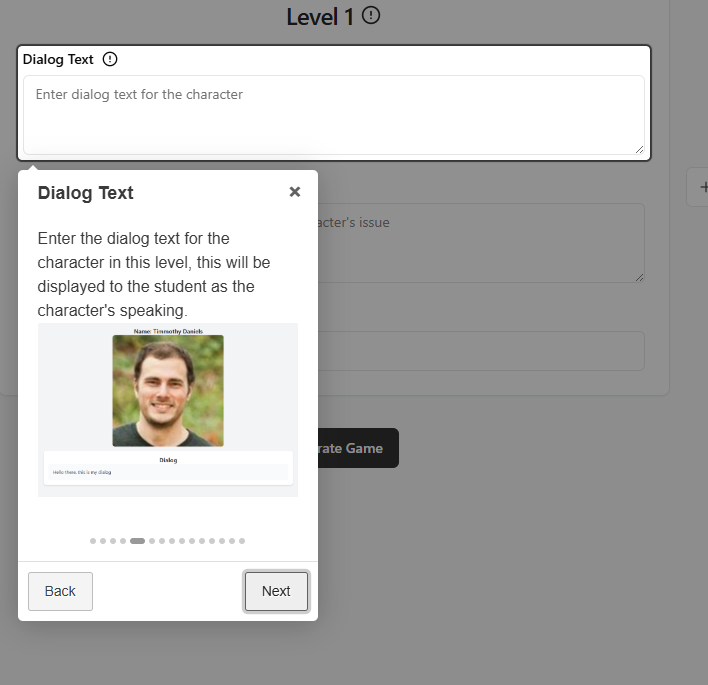
\includegraphics[width=0.8\textwidth]{figures/Diagnose_Game/Instructor_Portal_Diagnose_Game_hint.png}
    \caption{The tutorial system that was added to the platform after the focus group session.}
    \label{fig:tutorial}
\end{figure}

\begin{figure}
    \centering
    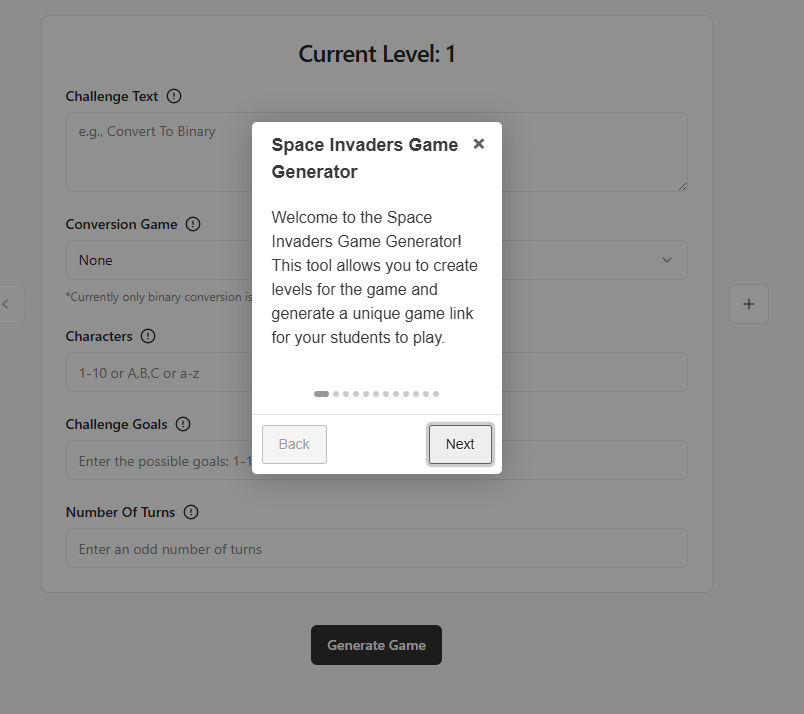
\includegraphics[width=0.8\textwidth]{figures/Space_Invaders/Instructor_Portal_Space_Invader_hint.png}
    \caption{The new design of the platform after the focus group session.}
    \label{fig:hint}
\end{figure}

\begin{figure}
    \centering
    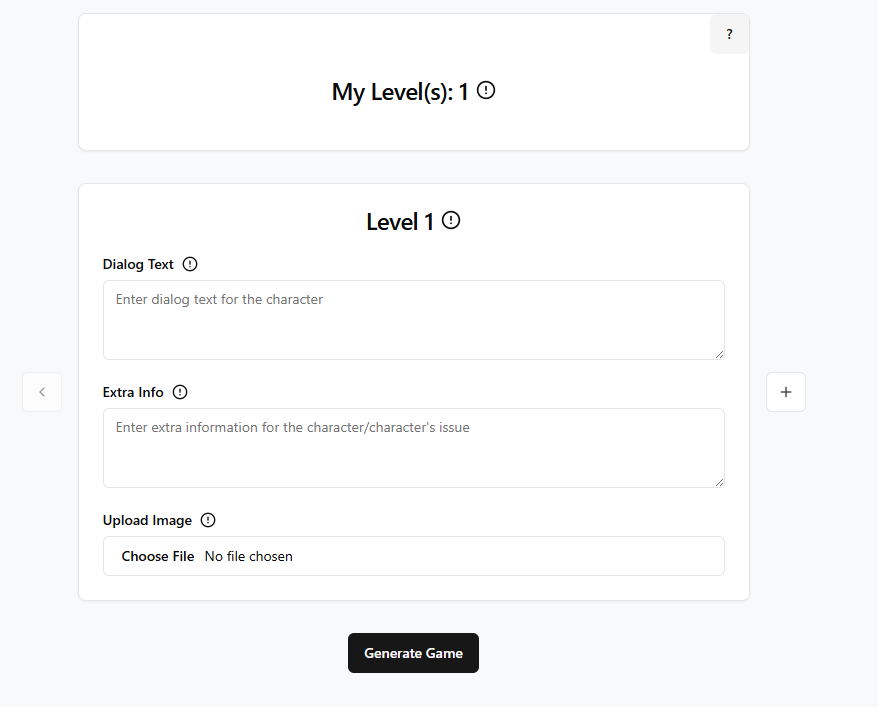
\includegraphics[width=0.8\textwidth]{figures/Diagnose_Game/Instructor_Portal_Diagnose_Game.png}
    \caption{The new design of the platform after the focus group session.}
    \label{fig:design}
\end{figure}

\section{Usability Study}

The usability study was conducted to evaluate the platform's ease of use, effectiveness, and overall user experience. twelve educators from the German International University (GIU) Computer Science department participated in the study. Each participant was asked to complete a series of tasks on the platform, such as creating a game, customizing game templates, and navigating through the platform's features. After completing the tasks, participants filled out a questionnaire to provide feedback on their experience. The platform was distributed to the participants via an email which included a link to the platform and a survey to fill out after the completion of the tasks. The participants were given a week to complete the tasks and fill out the survey. The usability study was conducted over a week, with participants completing the tasks at their convenience.

\section{Usability Study Results}
The survey measured Task Load Index (TLX) and System Usability Scale (SUS) scores, Immersion and Engagement scores, and overall user satisfaction. The results of the usability study are shown in Table \ref{tab:usability}. The participants rated the platform's ease of use, effectiveness, and overall user experience. The participants found the platform easy to use, with an average SUS score of 82.92. The participants also rated the platform's effectiveness and overall user experience highly, with an average score of 4.5 out of 5. The participants reported high levels of immersion and engagement with the platform, with an average score of 4.2 out of 5. The participants were satisfied with the platform overall, with an average score of 4.3 out of 5. The participants also reported low levels of task load, with an average TLX score of 3.13 out of 10. The results of the usability study indicate that the platform is easy to use, effective, and provides a positive user experience.

% Task load: [3.4, 3.4, 2.2, 4.6, 3.0, 2.4, 2.8, 2.6, 4.0, 3.0, 2.6, 3.6]
% SUS: [[92.5, 52.5, 97.5, 57.5, 85.0, 85.0, 77.5, 70.0, 100.0, 92.5, 100.0, 85.0]

\begin{table}[]
    \centering
    \begin{tabular}{|c|c|}
    \hline
    \textbf{Metric} & \textbf{Score} \\ \hline
    SUS & 82.92 \\ \hline
    Immersion and Engagement & 4.2 \\ \hline
    Overall User Satisfaction & 4.3 \\ \hline
    Task Load Index (TLX) & 3.13 \\ \hline
    \end{tabular}
    \caption{Usability Study Results}
    \label{tab:usability}
\end{table}